\section{Methods} % (~25%)
% It is always a good idea to write down your methods in detail, with all parameters written down, in a permanent place (e.g., a hard-backed book), while you are still doing the work, and to label all results with which experiment they belong to. Of course, if you will be working on computer, take back-ups seriously. Ideally, your report should contain enough information about the methods used to enable another student/researcher to replicate your experiments. The methods section should concisely describe your design as well as its materials and fabrication. Also specify which control strategy you are using for your robot and in case you are using a bioinspired design or another inspiration, state which animal(s)/character(s) it is inspired by and how. Lastly, describe the methodology of your human-robot interaction (HRI) experiment (procedure, measures/questions posed etc.).

\subsection{Fabrication}

\begin{figure}[!ht]
    \centering
    \includegraphics[width=0.9\linewidth]{data/cyc_bot_section.png}
    \caption{CycBot section view showing internal components and silicone parts.}\label{fig:cycbot-section}
\end{figure}

\par The~hardest part of CycBot to make, was the~silicone belly. We designed and 3D printed a~mold shown in Figure~\ref{fig:forma-cyca}. The~mold consists of four parts: split outer shell, inner core and cap to hold the~inner core in place. The~first step in making the~silicone belly was to assemble the~mold by~placing the inner core inside the outer shells, and securing it with the~cap. Then, we sealed all edges with duct tape to prevent silicone leakage. Because of the~wall thickness of the~belly (3~mm on the walls and 8~mm on the~bottom) and the~mold being relatively tall, we were concerned about air bubbles getting trapped inside the~silicone during pouring, which would make our part faulty. To keep our silicone bubble free, we put our silicone mixture in a~vacuum chamber for 15~minutes and then poured it slowly into the~mold through a~small hole on the~top of the~mold cap. After pouring, we placed the~mold in a~vacuum pot for 45~minutes to further eliminate any remaining air bubbles.

\par Fortunately, our part came out bubble-free on the~first try. We then placed the~mold in an~oven at~60$^\circ$C for 2~hours to cure the~silicone. We put our mold in the~oven for longer than recommended by the~silicone manufacturer to make sure the~silicone was fully cured, because 3D~printed molds tend to absorb some heat during the~curing process.

\par After curing, we disassembled the~mold and removed the~silicone belly. The~final step was to trim any excess silicone and glue the~belly to the~robot frame using Sil-Poxy silicone adhesive. Figure~\ref{fig:cycbot-section} shows a~section view of the~CycBot with all internal components and silicone parts.

\par In the~end our mold design worked very well, and we were able to make a~high quality silicone belly for our robot.

\begin{figure}[!ht]
    \centering
    \includegraphics[width=0.9\linewidth]{data/forma_cyca.png}
    \caption{3D~model of mold used to cast CycBot's silicone belly.}\label{fig:forma-cyca}
\end{figure}

% TODO: Add something about ears

\subsection{Hardware and software}

\par The~robot is controlled by the~Arduino~Uno microcontroller, equipped with a~motor shield~\cite{motor-shield}. The~motor shield has only 4~motor outputs, so it was a limiting factor for the~design. That meant, there could be only 4~pumps/valves used for robot the~actuation. The~code used in this project can be found on~\href{https://github.com/AlanBejnarowicz/CycBot}{GitHub}.

\begin{figure}[!ht]
    \centering
    \includegraphics[width=0.75\linewidth]{data/cables.jpg}
    \caption{Processing unit hidden inside the robot's base.}\label{fig:cables}
\end{figure}

\par The~final design incorporates 3~air pumps, 2~solenoid valves, 1~servo motor and 1~differential pressure sensor. The~power source is a~5.9~V, 2~A power adapter, but, as it turned out not to be enough, the~Arduino board has to be powered separately via USB cable. To overcome the~limited number of motor outputs, the 2~solenoid valves share the~same motor output of the~motor shield. Because of that, the~robot's ears could not be deflated independently.

\par The first pump, is responsible for the belly inflation. It is coupled in the feedback loop with the pressure sensor. Its readings are read by~the~Arduino's ADC and filtered using an~alpha-beta digital filter~\cite{alpha-beta-filter}. Then, they are used by~the~PI~controller to maintain the~desired air pressure inside the~belly.

\par Additionally, sudden changes in pressure readings can be detected, and counted as touches. Timers are used to distinguish between the~short and long presses. After a~touch is detected, the~dead zone timer is started to prevent multiple touch detections from a~single press.

\par The~other two pump are responsible for inflating the robot's ears. The ears can be inflated independently, but as they are connected through the~solenoid valves to the~same motor shield output, they can only be deflated simultaneously. There are also no pressure sensor for the ears, so they have to be controlled by a feed-forward controller.

\par The~servo motor is used to move the~robot's head. It is powered directly from the~power adapter to avoid voltage drops on the~microcontroller.

\subsection{Robot's behaviour}

\begin{table}[!ht]
    \caption{Robot expressed emotions.}\label{tab:emotions}
    \begin{center}
        \begin{tabular}{ccccc}
            \hline
            Emotion & \multicolumn{1}{c}{Ears movement} & \multicolumn{1}{c}{Head movement} \\
            \hline
            Sad & Both ears down & --- \\
            Interested & --- & Slow head swipe \\
            Happy & Move both ears one at a~time & --- \\
            Annoyed & --- & Rapid head movements \\
            \hline
        \end{tabular}
    \end{center}
\end{table}

\par The~robot operates based on a~state machine that defines interactions with humans (see Table~\ref{tab:emotions} and Table~\ref{tab:state-changes}). The~robot starts in the~default, sad state (see Figure~\ref{fig:cycbot-sad}), where it waits for human interaction. Both ears are inflated to point downwards, indicating sadness. When a~single short touch is detected, the~robot transitions to the~interested state (see Figure~\ref{fig:cycbot-interested}), where it slowly swipes its head side to side, showing curiosity. If no interaction occurs for 20~seconds, the~robot returns to the~sad state.

\begin{figure}[!ht]
    \centering
    \begin{subfigure}{0.49\linewidth}
        \centering
        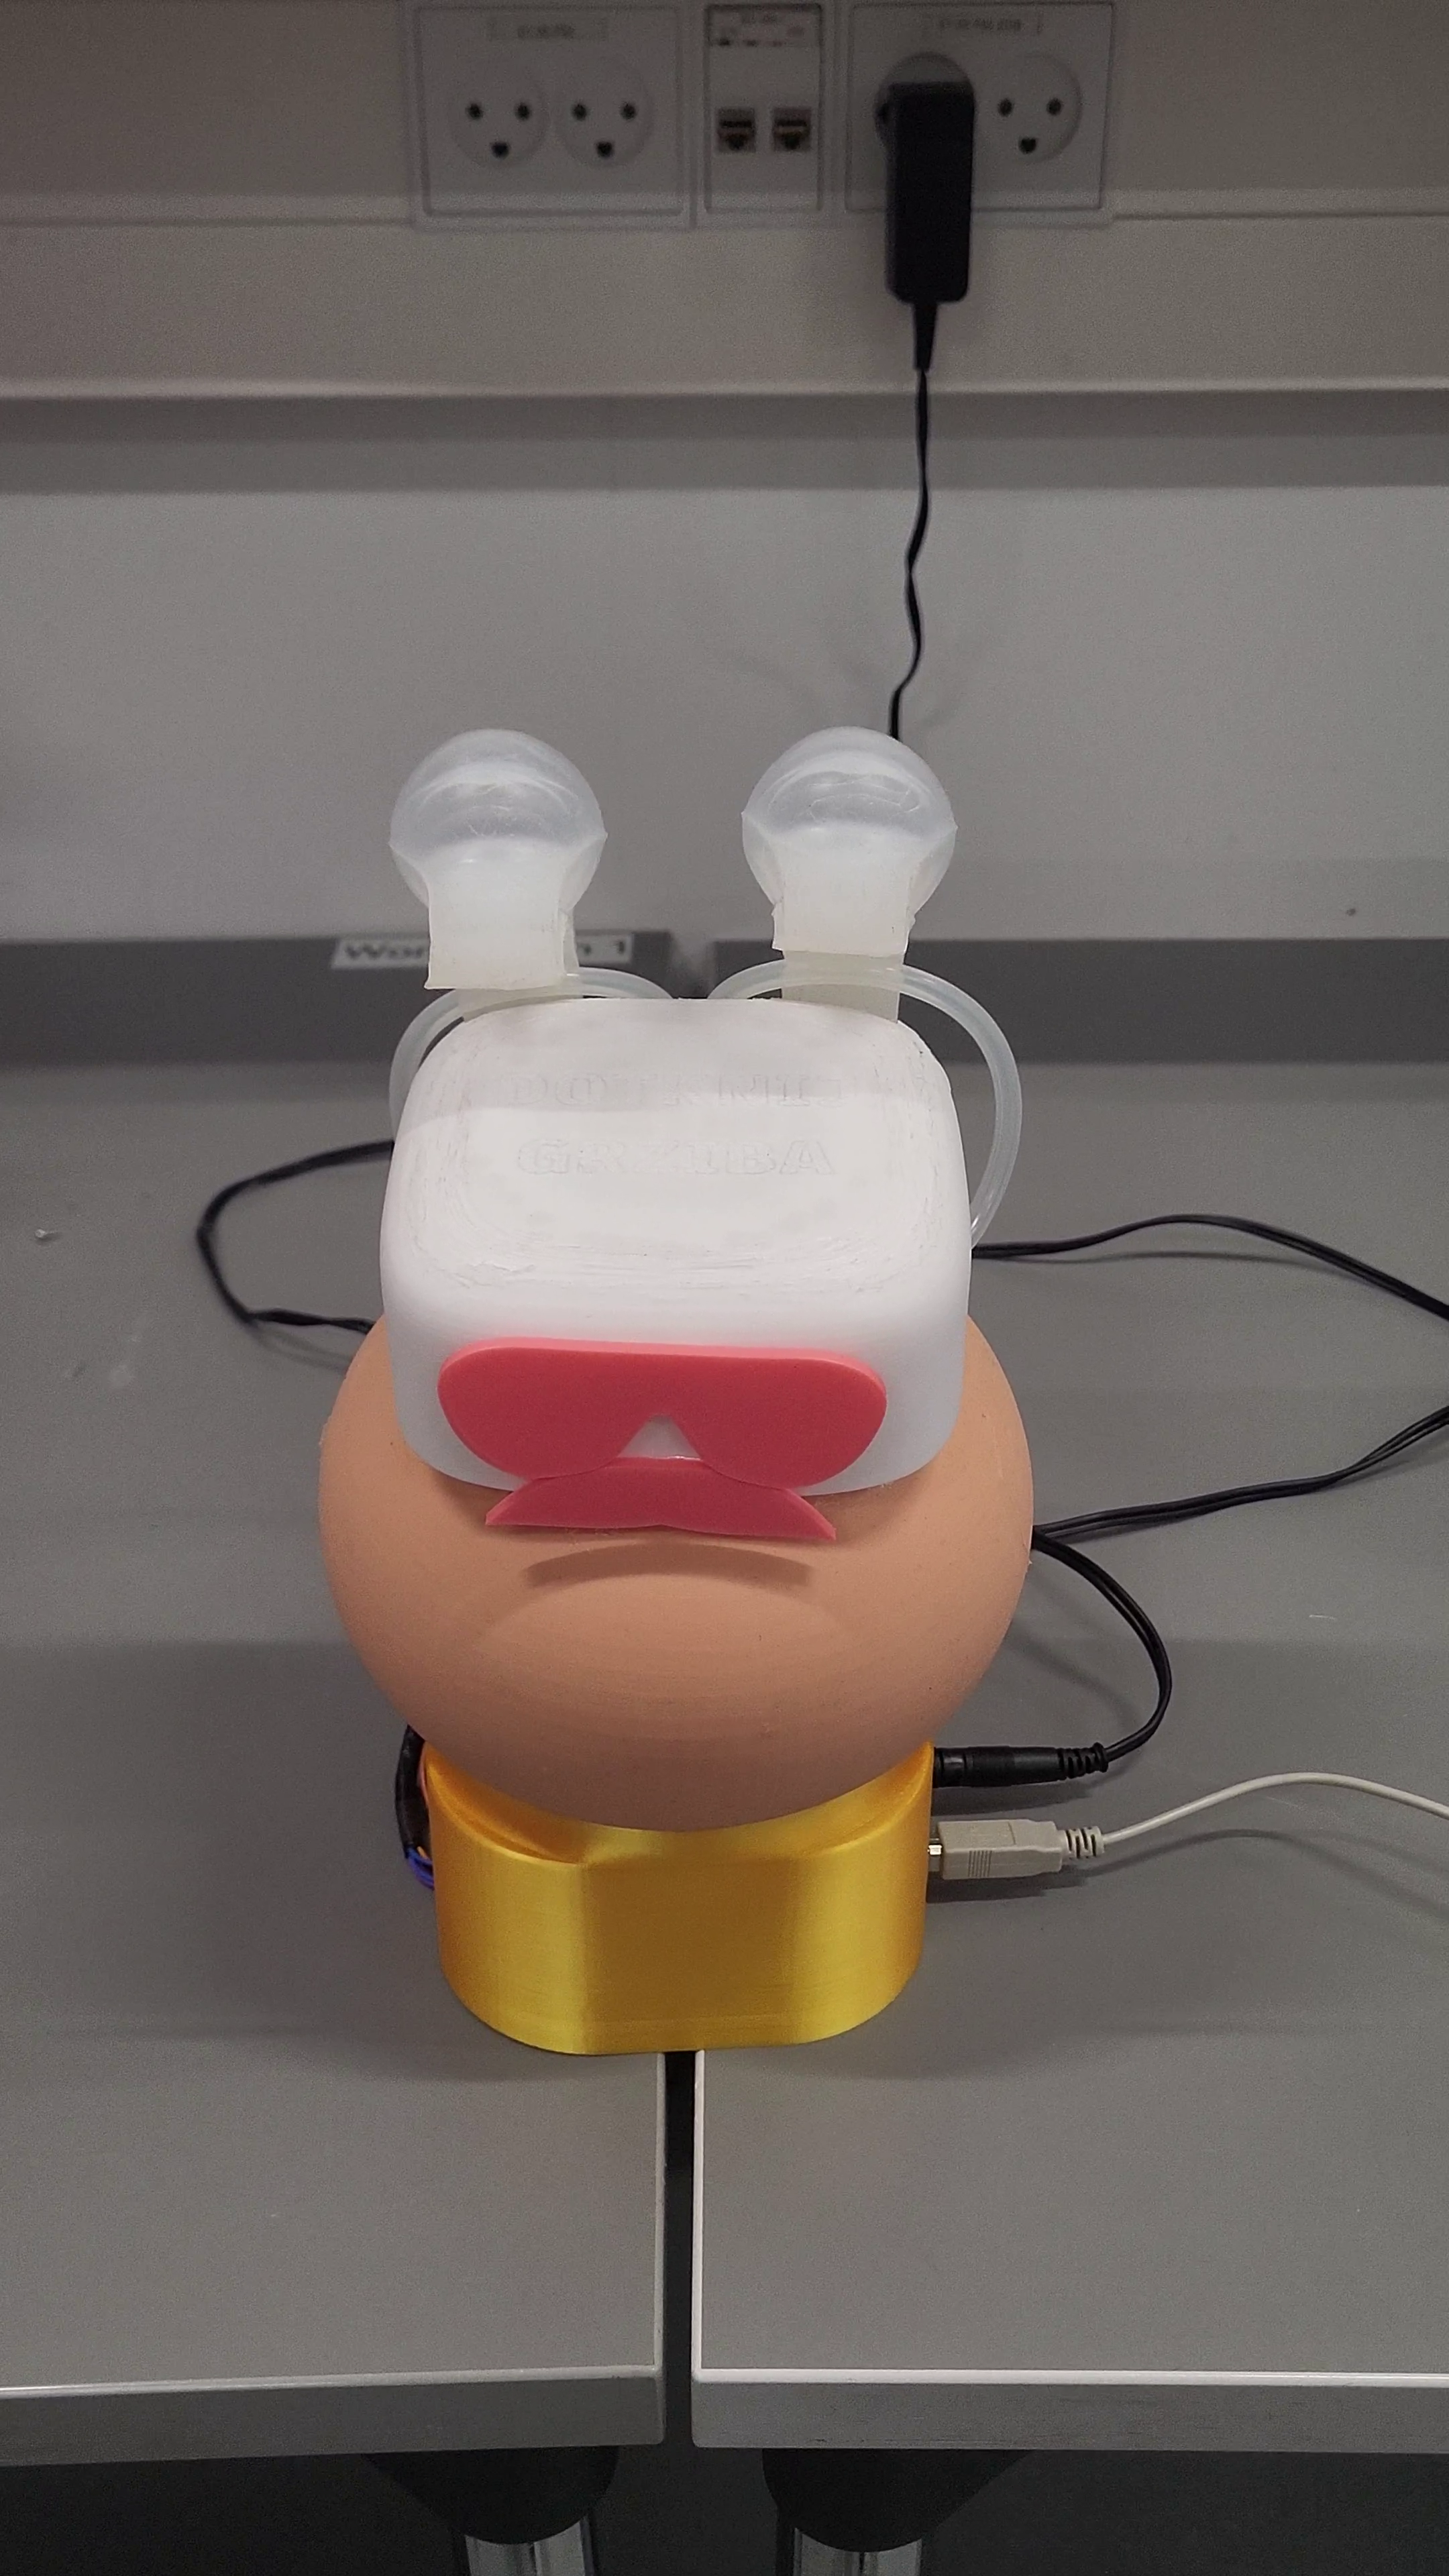
\includegraphics[width=\linewidth]{data/sad.png}
        \caption{Sad state.}\label{fig:cycbot-sad}
    \end{subfigure}
    \hfill
    \begin{subfigure}{0.49\linewidth}
        \centering
        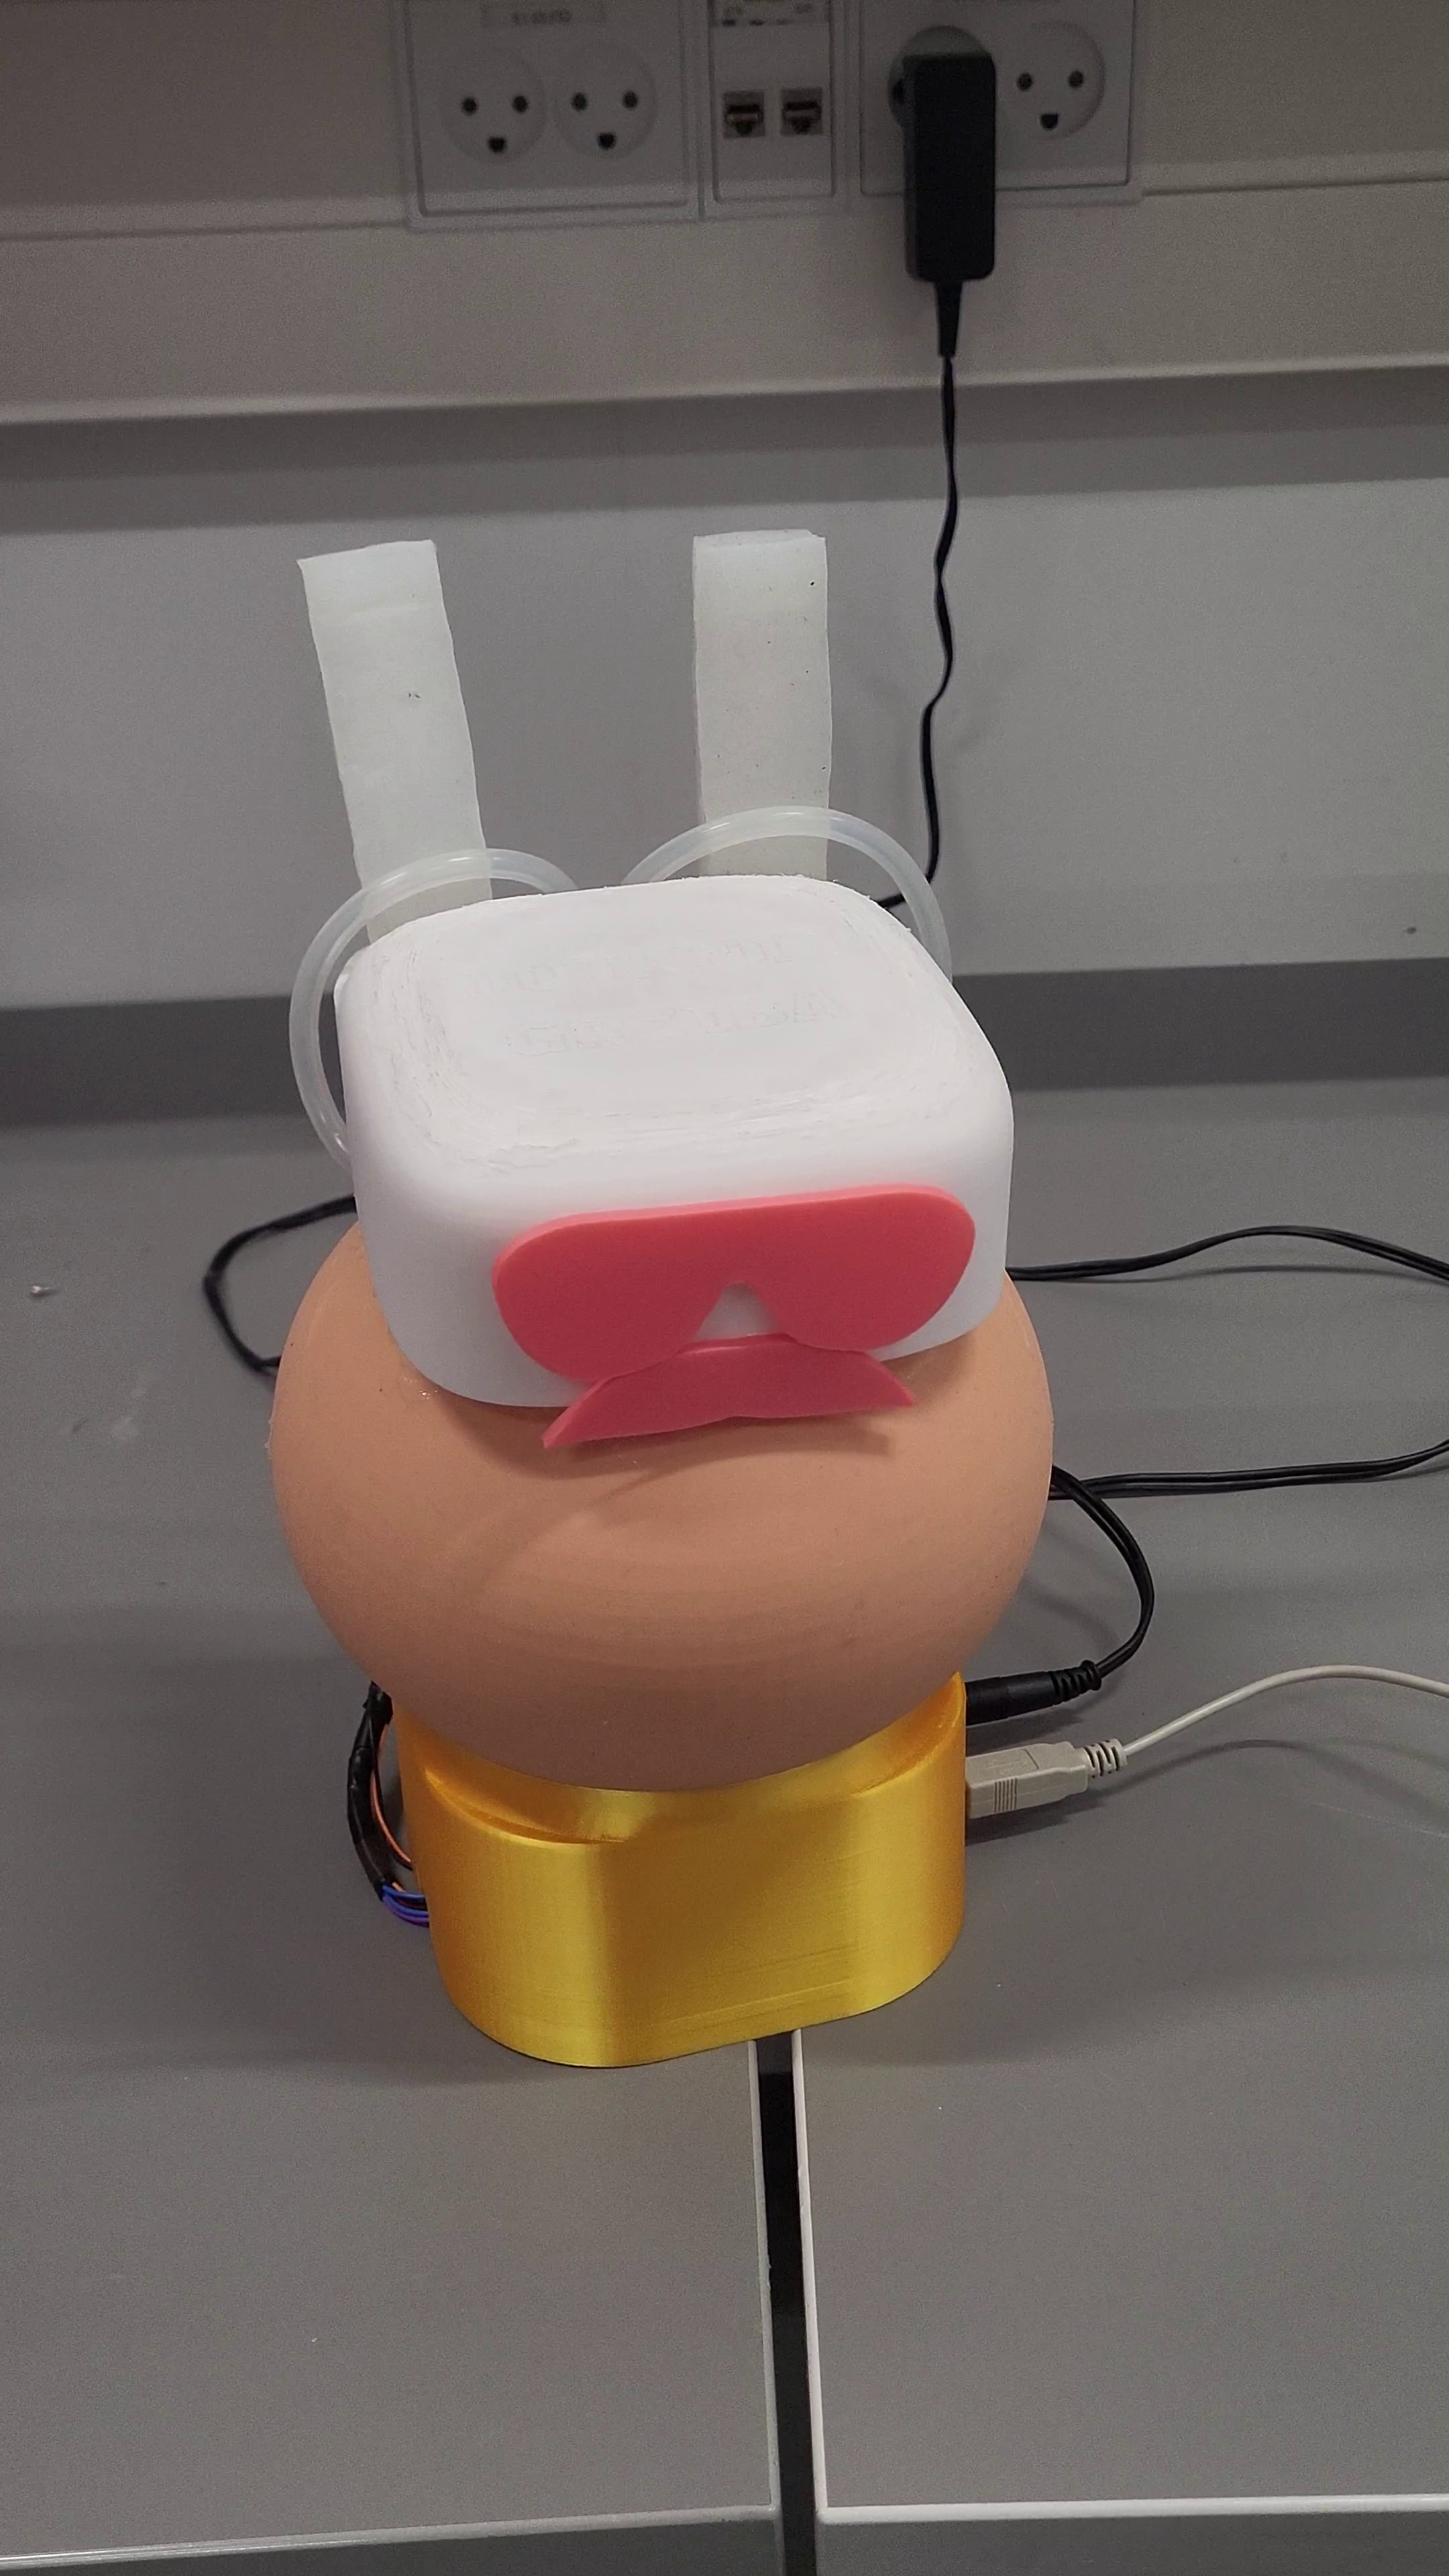
\includegraphics[width=\linewidth]{data/interested.png}
        \caption{Interested state.}\label{fig:cycbot-interested}
    \end{subfigure}
    \caption{CycBot in different emotional states.}\label{fig:cycbot-emotions-1}
\end{figure}

\par A~single short touch in the~interested state makes the~robot happy (see Figure~\ref{fig:cycbot-happy}). In this state, the~robot moves its ears one at a~time, expressing joy. If no interaction occurs for 20~seconds, the~robot goes back to the~sad state. However, if a~double or long touch is detected while happy, the~robot becomes annoyed (see Figure~\ref{fig:cycbot-annoyed}). In this state, it rapidly moves its head side to side, indicating irritation. After 10~seconds, the~robot calms down and returns to the~interested state.

\begin{figure}[!ht]
    \centering
    \begin{subfigure}{0.49\linewidth}
        \centering
        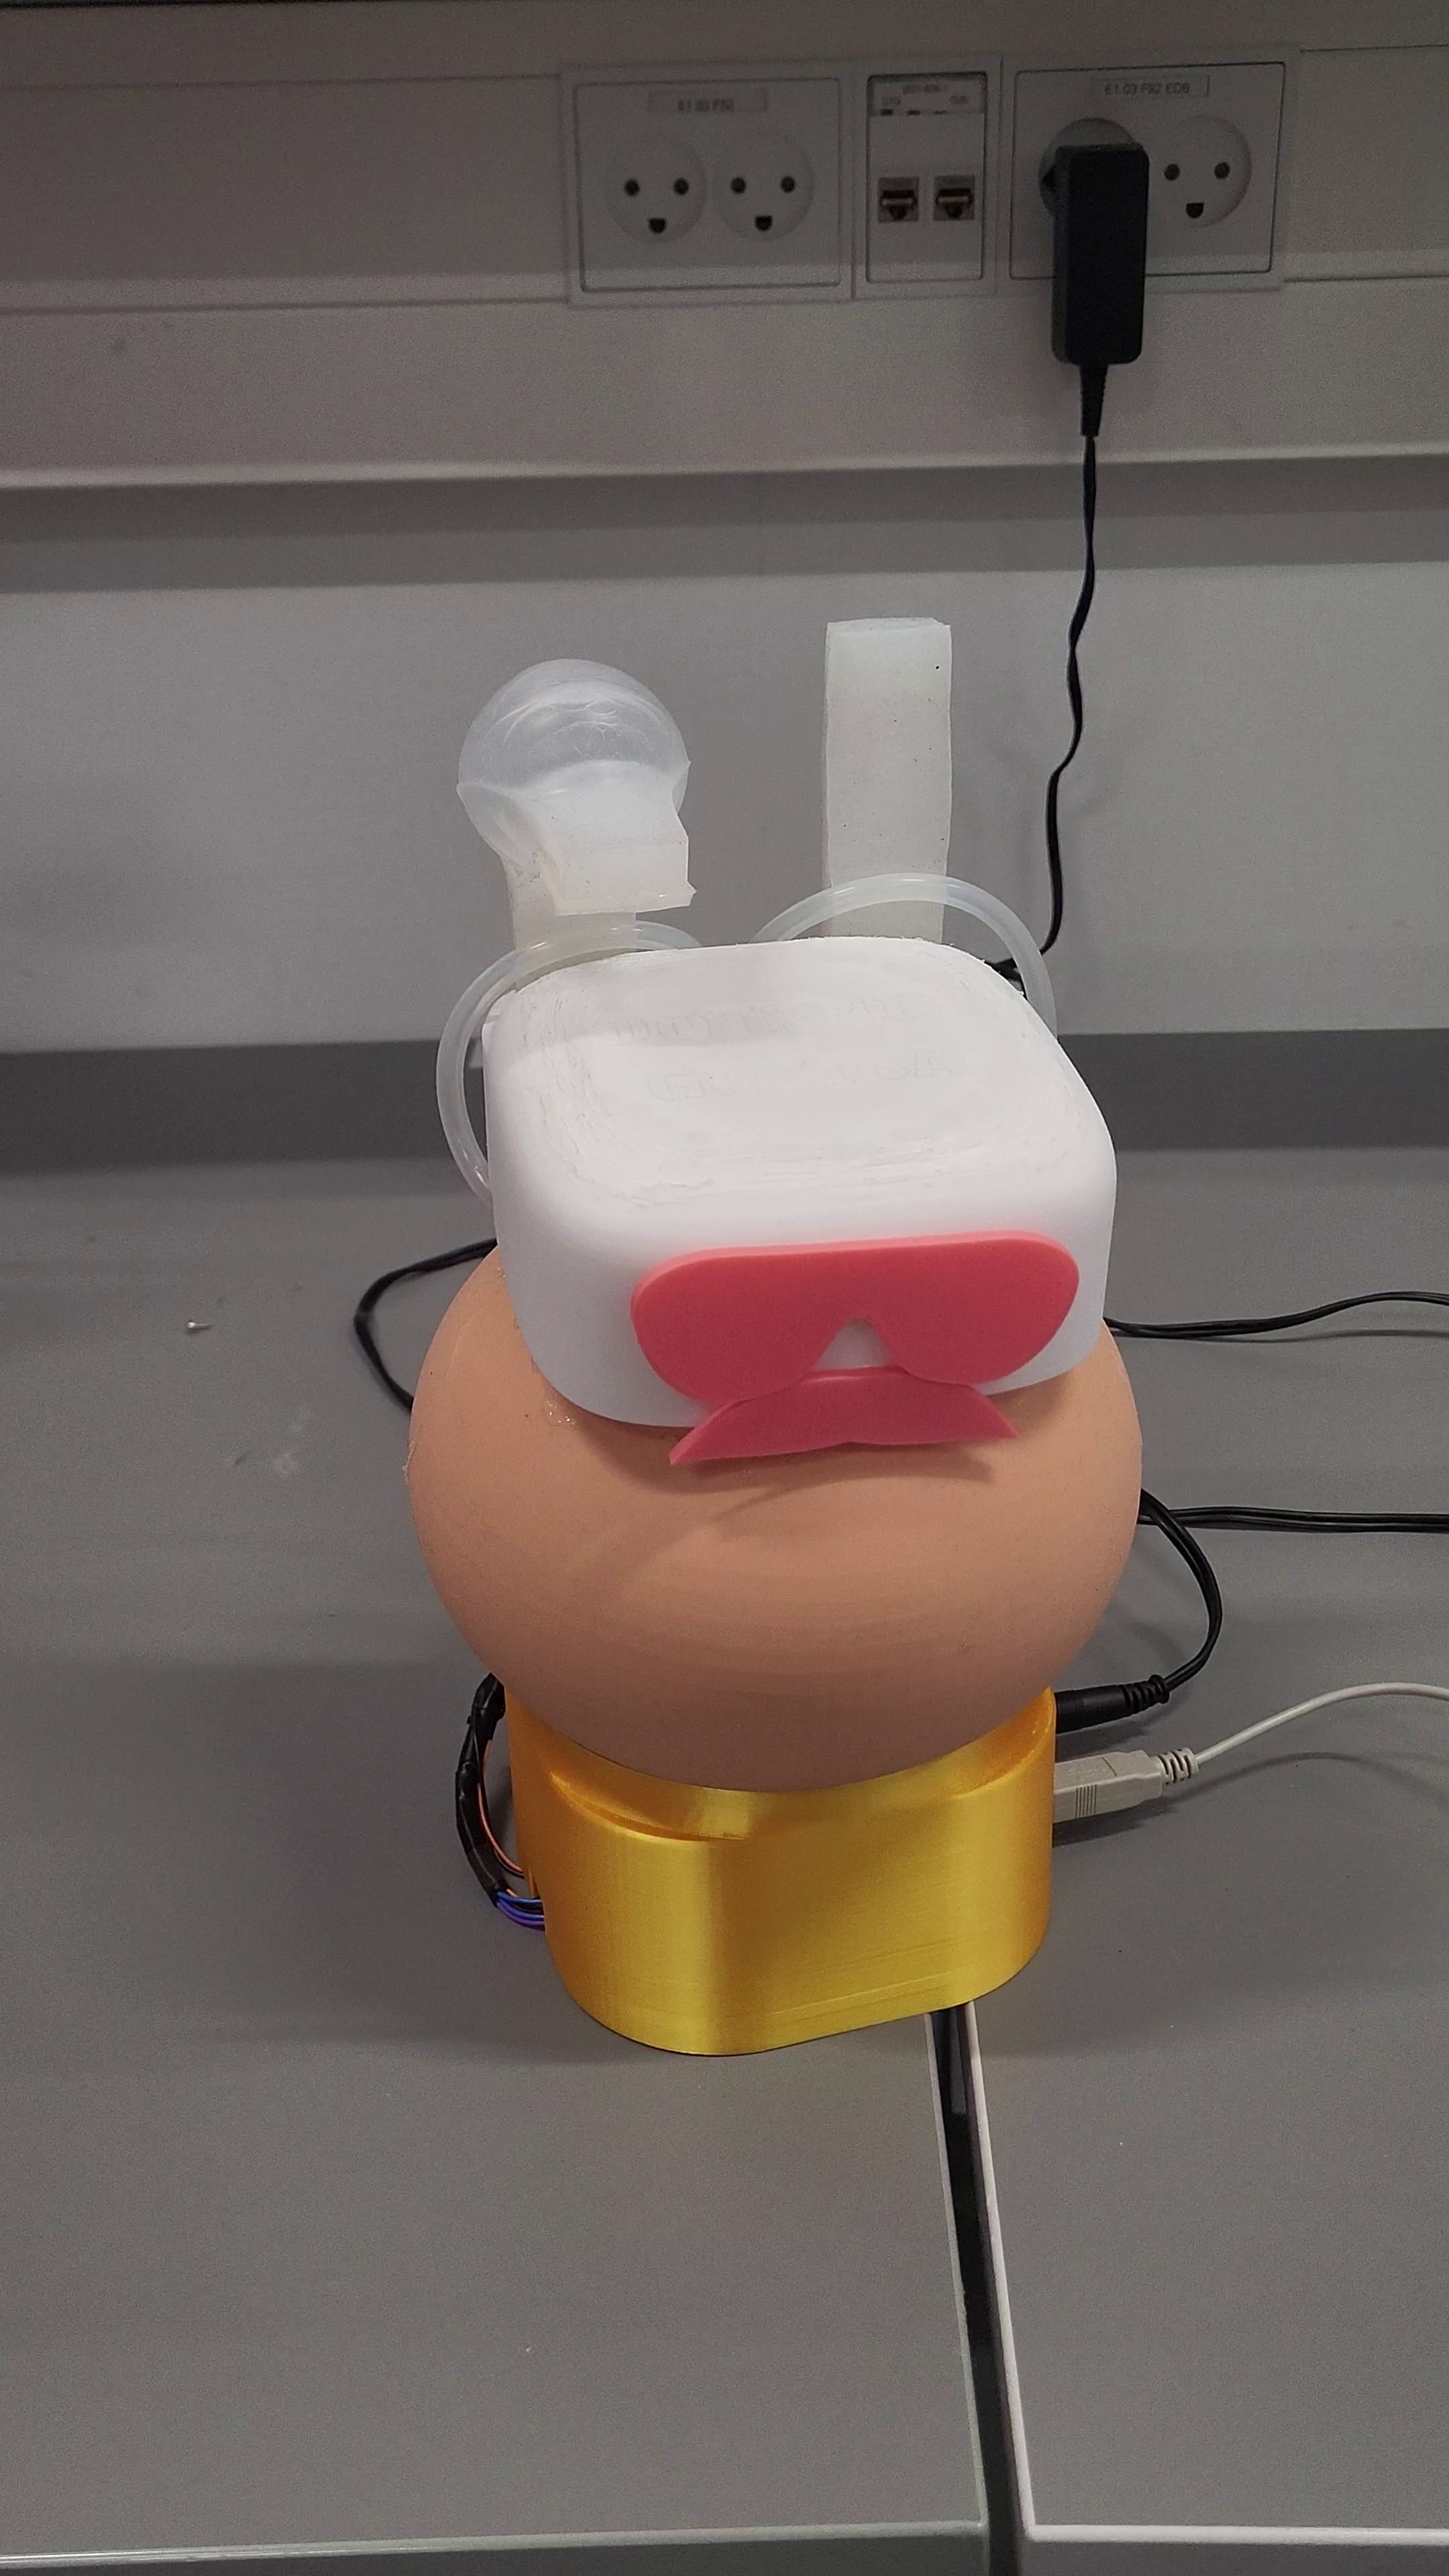
\includegraphics[width=\linewidth]{data/happy.png}
        \caption{Happy state.}\label{fig:cycbot-happy}
    \end{subfigure}
    \hfill
    \begin{subfigure}{0.49\linewidth}
        \centering
        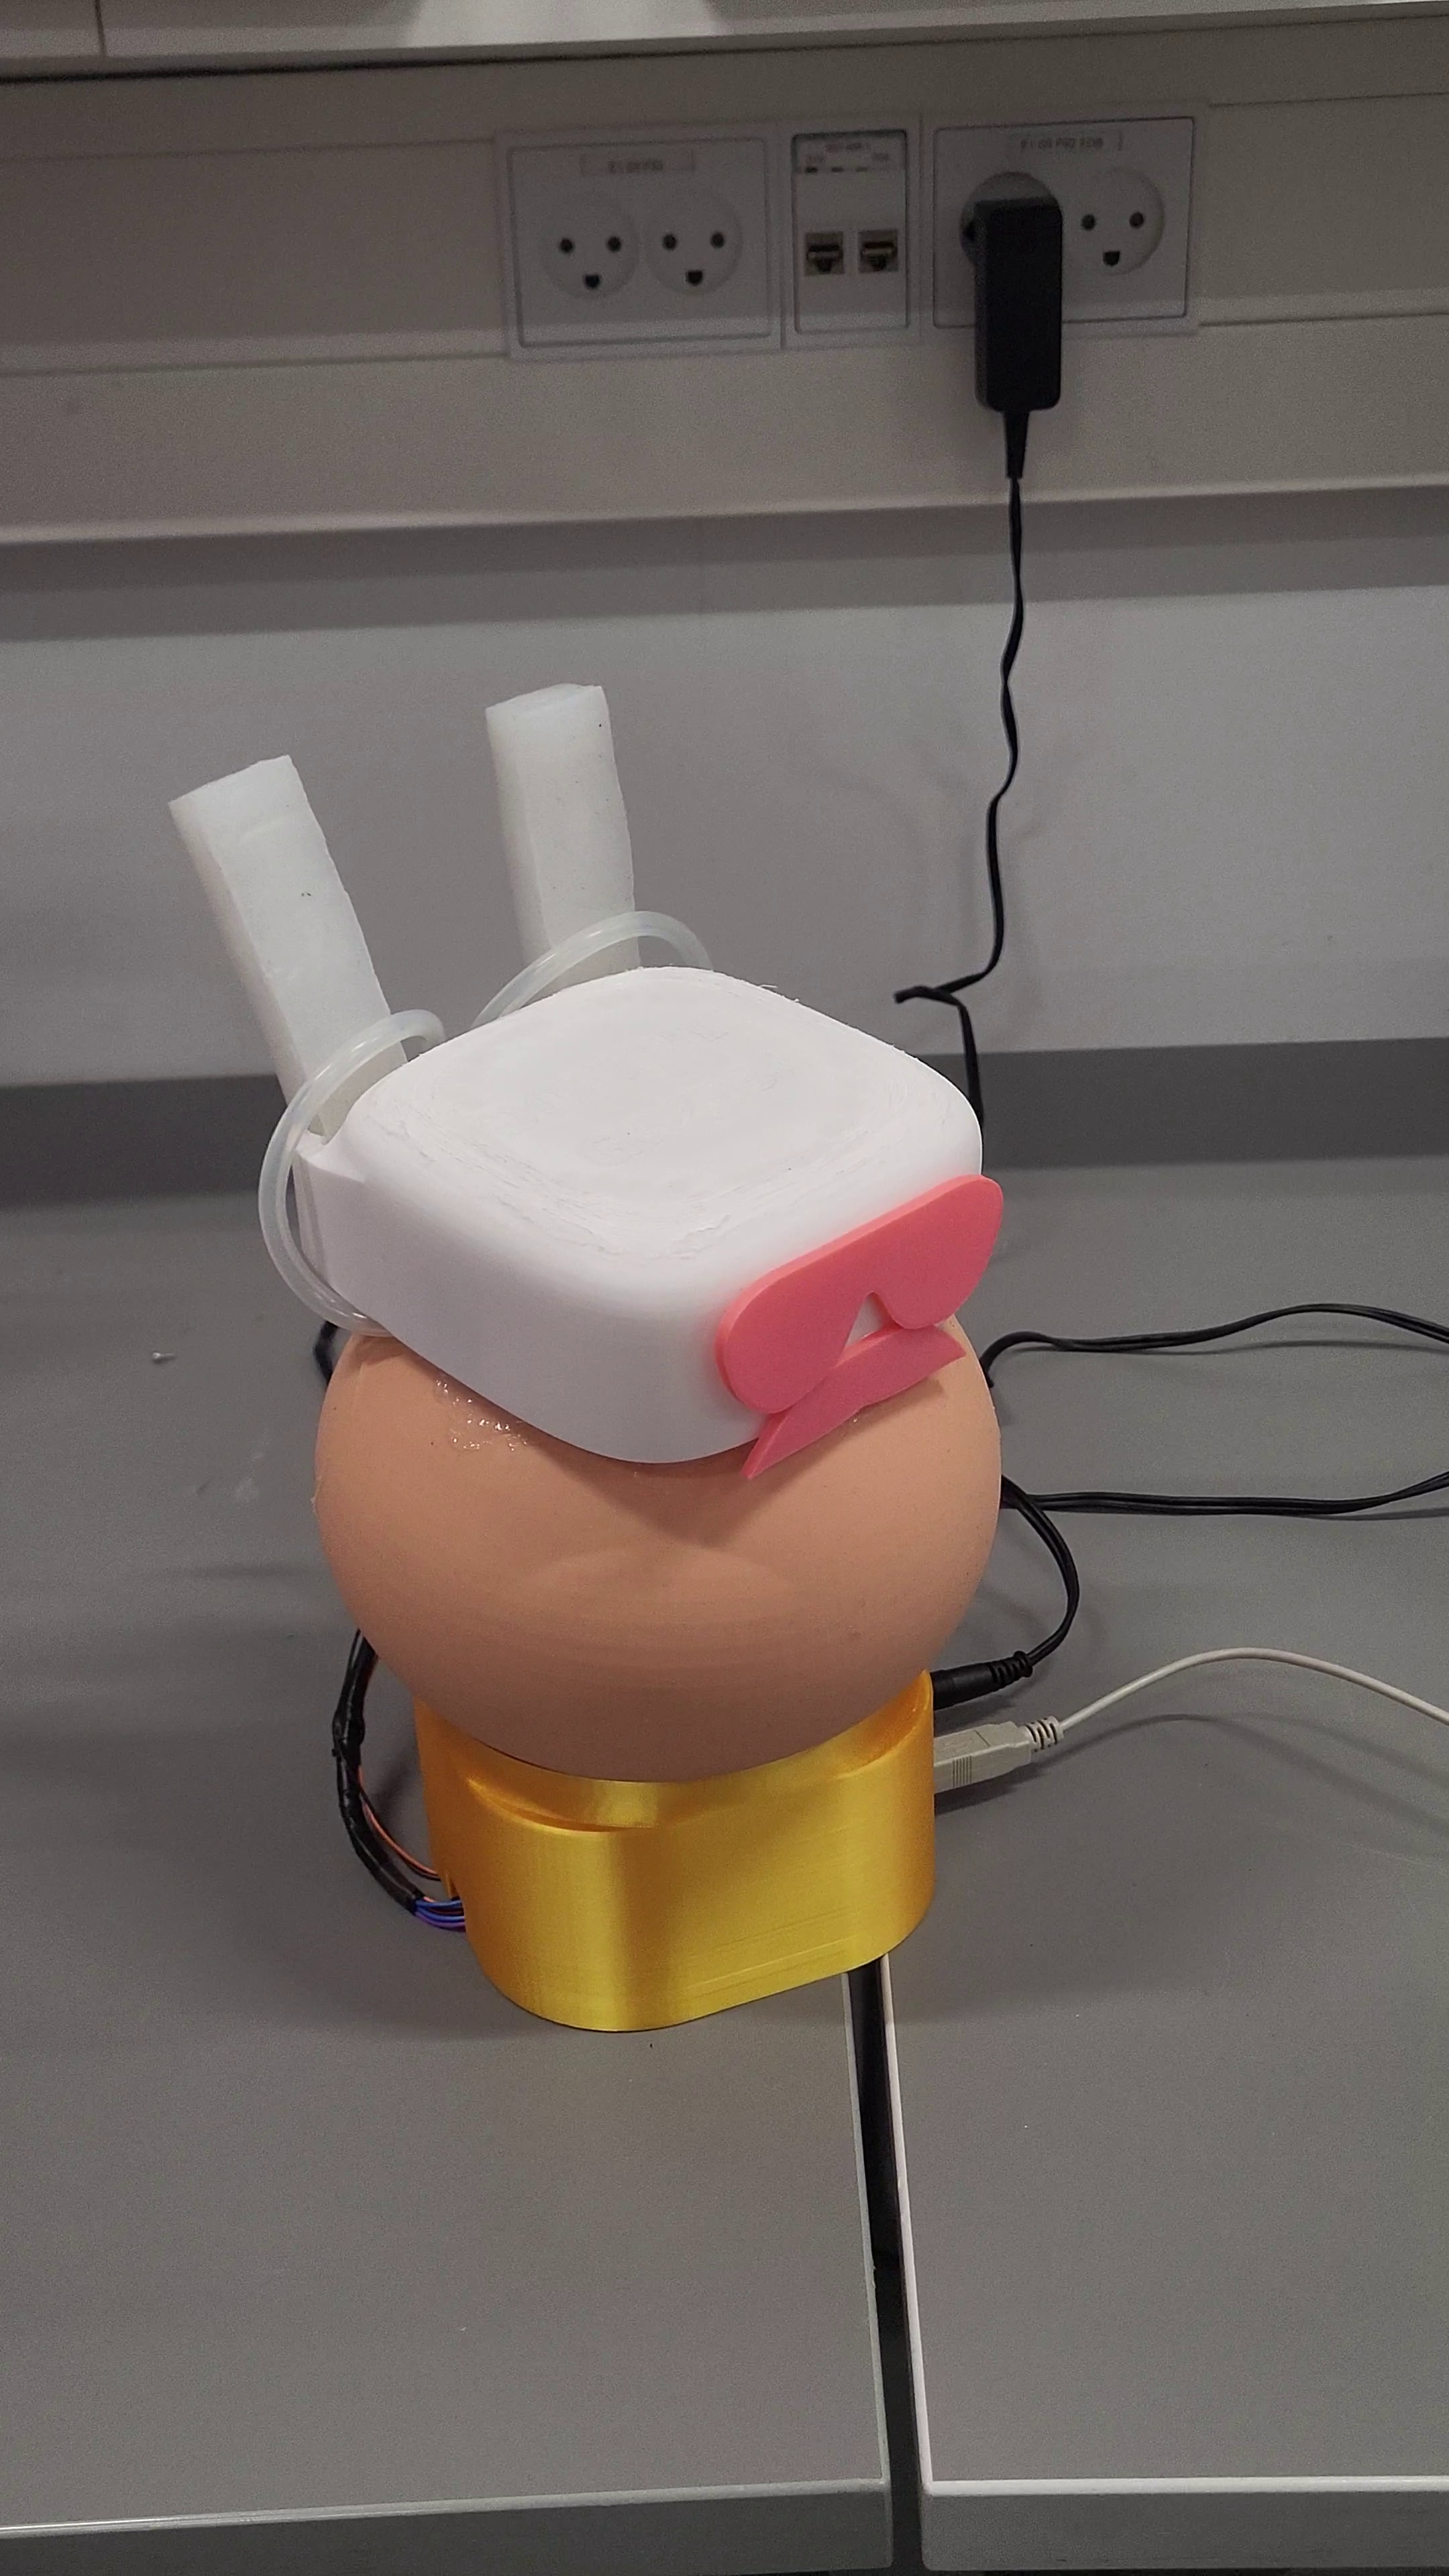
\includegraphics[width=\linewidth]{data/annoyed.png}
        \caption{Annoyed state.}\label{fig:cycbot-annoyed}
    \end{subfigure}
    \caption{CycBot in different emotional states.}\label{fig:cycbot-emotions-2}
\end{figure}

\begin{table}[!ht]
    \caption{State changes.}\label{tab:state-changes}
    \begin{center}
        \begin{tabular}{cc}
            \hline
            State change & Cause \\
            \hline
            Sad $\rightarrow$ Interested & Single short touch \\
            Interested $\rightarrow$ Sad & No interaction for 20~s \\
            Interested $\rightarrow$ Happy & Single short touch \\
            Happy $\rightarrow$ Sad & No interaction for 20~s \\
            Happy $\rightarrow$ Annoyed & Double or long touch \\
            Annoyed $\rightarrow$ Interested & After 10~s \\
            \hline
        \end{tabular}
    \end{center}
\end{table}

\par The state machine design is also shown in Figure~\ref{fig:cycbot-state}.

\begin{figure}[!ht]
    \centering
    \includegraphics[width=0.9\linewidth]{data/cyc_state_machine.png}
    \caption{CycBot state machine diagram.}\label{fig:cycbot-state}
\end{figure}

\subsection{HRI experiment}

\par Signals used in experiments are robot behaviours explained in Table~\ref{tab:emotions}.

\textbf{Hypothesis H1:} Participants will touch robot more while presenting Interested or Annoyed expression.
\textbf{Measure:} Number of touches during each behaviour.
\textbf{Analysis:} One-way ANOVA test to compare means of touches during each behaviour.
